\documentclass[11pt]{article}

\usepackage[a4paper,margin=2.5cm]{geometry}
\usepackage[utf8]{inputenc}
\usepackage[T2A, T1]{fontenc}
\usepackage[ukrainian,english]{babel}
\usepackage{amsmath,amssymb}
\usepackage{graphicx}
\usepackage{hyperref}
\usepackage{listings}
\usepackage{xcolor}

% Monospace font for code, type names, functions, etc.
\usepackage{inconsolata}
\newcommand{\code}[1]{\texttt{#1}}

\usepackage{newunicodechar}
\newunicodechar{ʼ}{'}

% Big-O and big-Theta notation
\newcommand{\BigO}[1]{\mathcal{O}(#1)}
\newcommand{\BigTheta}[1]{\Theta(#1)}

\lstset{
    basicstyle=\ttfamily\small,
    breaklines=true,
    frame=single,
    columns=fullflexible,
    backgroundcolor=\color{gray!10},
    keywordstyle=\color{blue},
    commentstyle=\color{gray},
    stringstyle=\color{teal},
}

\lstdefinelanguage{Rust}{
    keywords={as,break,const,continue,else,enum,fn,for,if,impl,in,let,loop,match,mod,mut,pub,return,self,Self,struct,use,where,while},
    sensitive=true,
    comment=[l]{//},
    string=[b]",
}

\lstdefinestyle{ruststyle}{
    language=Rust,
    basicstyle=\ttfamily\footnotesize,
    numbers=left,
    numberstyle=\tiny\color{gray},
    numbersep=8pt,
    tabsize=4,
    showstringspaces=false,
    frame=single,
    breaklines=true,
    columns=fullflexible,
    backgroundcolor=\color{gray!10},
    keywordstyle=\color{blue!70!black}\bfseries,
    commentstyle=\color{gray},
    stringstyle=\color{teal},
}

\title{Спеціальні розділи обчислювальної математики\\
Компʼютерний практикум №1\\[1em]
Багаторозрядна арифметика}
\author{ФІ-43 Редько Микита}
\date{\today}

\begin{document}
\selectlanguage{ukrainian}

\maketitle

\section{Мета роботи}
Отримання практичних навичок програмної реалізації багаторозрядної арифметики;
ознайомлення з прийомами ефективної реалізації критичних по часу ділянок
програмного коду та методами оцінки їх ефективності.

\section{Результати}

Нижче наведено тести для основних операцій багаторозрядної арифметики.
Їх успішне виконання засвідчує коректність нашої імлементації.
\subsection{Перетворення чисел}

Перевіряються перетворення малих констант (u64), перетворення рядка з шістнадцятковим числом та зворотне перетворення числа у рядок.

\begin{lstlisting}[style=ruststyle]
#[test]
fn test_u64_to_big_int_zero() {
    let expected = BigInt {
        limbs: [0; BIG_INT_LIMBS],
    };

    assert_eq!(u64_to_big_int(0), expected);
}

#[test]
fn test_u64_to_big_int_value() {
    let mut limbs = [0; BIG_INT_LIMBS];
    limbs[0] = 91726;
    let expected = BigInt { limbs };

    assert_eq!(u64_to_big_int(91726), expected);
}

#[test]
fn test_hex_to_big_int_multiple() {
    let value = hex_to_big_int("1000000000000123A").unwrap();

    assert_eq!(big_int_to_hex(&value), "1000000000000123A");
}

#[test]
fn test_big_int_to_hex_single() {
    let mut limbs = [0u64; BIG_INT_LIMBS];
    limbs[0] = 0x123A;
    let number = BigInt { limbs };

    assert_eq!(big_int_to_hex(&number), "123A");
}
\end{lstlisting}

\subsection{Порівняння, додавання та віднімання}

Тести перевіряють результати порівняння, перенесення під час додавання, віднімання з запозиченням та випадок, коли результат віднімання є відʼємним.

\begin{lstlisting}[style=ruststyle]
#[test]
fn test_cmp_equal() {
    let a = u64_to_big_int(7);
    let b = u64_to_big_int(7);

    assert!(matches!(compare_big_int(&a, &b), Comparison::Equal));
}

#[test]
fn test_cmp_less() {
    assert!(matches!(
        compare_big_int(&u64_to_big_int(6), &u64_to_big_int(7)),
        Comparison::Less
    ));
}

#[test]
fn test_cmp_greater() {
    assert!(matches!(
        compare_big_int(&u64_to_big_int(7), &u64_to_big_int(6)),
        Comparison::Greater
    ));
}

#[test]
fn test_add_big_int_carry() {
    let mut a_limbs = [0; BIG_INT_LIMBS];
    a_limbs[0] = u64::MAX;
    a_limbs[1] = 4;
    let a = BigInt { limbs: a_limbs };

    let mut b_limbs = [0; BIG_INT_LIMBS];
    b_limbs[0] = 1;
    b_limbs[1] = 2;
    let b = BigInt { limbs: b_limbs };

    let mut expected_limbs = [0; BIG_INT_LIMBS];
    expected_limbs[1] = 7;
    let expected = BigInt {
        limbs: expected_limbs,
    };

    assert_eq!(add_big_int(&a, &b), expected);
}

#[test]
fn test_subtract_success() {
    let a = hex_to_big_int("10000000000000000").unwrap();
    let b = u64_to_big_int(1);
    let expected = hex_to_big_int("FFFFFFFFFFFFFFFF").unwrap();

    assert_eq!(subtract_big_int(&a, &b), Some(expected));
}

#[test]
fn test_subtract_fail() {
    assert_eq!(
        subtract_big_int(&u64_to_big_int(1), &u64_to_big_int(2)),
        None
    );
}
\end{lstlisting}

\subsection{Множення та піднесення до квадрата}

Перевіряються множення двох багаторозрядних чисел, дистрибутивність множення відносно додавання, множення як повторне додавання, результат піднесення до квадрата та узгодженість квадрата з множенням числа на себе.

\begin{lstlisting}[style=ruststyle]
#[test]
fn test_mult_big_int() {
    assert_eq!(
        mult_big_int(
            &hex_to_big_int("ABCDEFEFFDFDDBCBDBAAAAACEEEEEEFEEFE").unwrap(),
            &hex_to_big_int("BABFAFBAEBAFEAFEAEF").unwrap()
        ),
        hex_to_big_int(
            "7D5444E99B6A6FD5AAA81359C0B5FFAC76C7A80AD34528C6164B22"
        )
        .unwrap()
    );
}

#[test]
fn test_mult_distributive_over_addition() {
    let a = hex_to_big_int("FEDCBA9876543210FFFFFFFFFFFFFFFF").unwrap();
    let b = hex_to_big_int("123456789ABCDEF0123456789ABCDEF0").unwrap();
    let c = hex_to_big_int("10000000000000001").unwrap();
    let sum = add_big_int(&a, &b);

    assert_eq!(
        mult_big_int(&sum, &c),
        add_big_int(&mult_big_int(&a, &c), &mult_big_int(&b, &c))
    );
}

#[test]
fn test_mult_by_repeated_addition() {
    let multiplier = u64_to_big_int(100);
    let value = hex_to_big_int("FFFFFFFFFFFFFFFF0000000000000001").unwrap();
    let mut sum = u64_to_big_int(0);

    for _ in 0..100 {
        sum = add_big_int(&sum, &value);
    }

    assert_eq!(mult_big_int(&multiplier, &value), sum);
}

#[test]
fn test_square_big_int() {
    let value = hex_to_big_int("ABCDEFEFFDFDDBCBDBAAAAACEEEEEEFEEFE").unwrap();
    let expected = hex_to_big_int(concat!(
        "734CC434C48FE970985A9A52515963D6E4643A",
        "2B2A625BDE8BBCB60B1C298865614404"
    ))
    .unwrap();

    assert_eq!(square_big_int(&value), expected);
}

#[test]
fn test_square_mult_consistency() {
    let value = hex_to_big_int("ABCDEFEFFDFDDBCBDBAAAAACEEEEEEFEEFE").unwrap();

    assert_eq!(square_big_int(&value), mult_big_int(&value, &value));
}
\end{lstlisting}

\subsection{Ділення та остача}

Окремо перевіряється ділення на нуль, ділення меншого числа на більше, більшого на менше. Для останніх двох випадків тест порівнює і
частку, і остачу.

\begin{lstlisting}[style=ruststyle]
#[test]
fn test_divide_mod_by_zero() {
    assert_eq!(
        divide_mod_big_int(&u64_to_big_int(10), &u64_to_big_int(0)),
        None
    );
}

#[test]
fn test_divide_mod_larger_by_smaller() {
    let a = hex_to_big_int(concat!(
        "AABABABABABABABABABABAABABABAAABABABABAB",
        "ABABABABABABABABABABAAABABAB"
    ))
    .unwrap();
    let b = hex_to_big_int("34234534645345324534564635345643563456343456").unwrap();

    assert_eq!(
        divide_mod_big_int(&a, &b),
        Some((
            hex_to_big_int("3464AFF4F01C1CA3B3320E2D812").unwrap(),
            hex_to_big_int("1C29AEB03271A65F72AF3C44D7B4CEE6937E9AEB6D9F").unwrap()
        ))
    );
}

#[test]
fn test_divide_mod_smaller_by_larger() {
    let a = hex_to_big_int("34234534645345324534564635345643563456343456").unwrap();
    let b = hex_to_big_int(concat!(
        "AABABABABABABABABABABAABABABAAABABABABAB",
        "ABABABABABABABABABABAAABABAB"
    ))
    .unwrap();

    assert_eq!(divide_mod_big_int(&a, &b), Some((u64_to_big_int(0), a)));
}
\end{lstlisting}

\subsection{Піднесення до степеня}

Тест звіряє результат піднесення багаторозрядного числа до степеня з наперед обчисленим значенням.

\begin{lstlisting}[style=ruststyle]
#[test]
fn test_horner_exponentiation() {
    let p = hex_to_big_int(
        "FFFFFFFFFFFFFFFFFFFFFFFFFFFFFFFFFFFFFFFFFFFFFFFFFFFFFFFEFFFFFC2F"
    )
    .unwrap();
    let exponent = u64_to_big_int(7);
    let expected = concat!(
        "FFFFFFFFFFFFFFFFFFFFFFFFFFFFFFFFFFFFFFFF",
        "FFFFFFFFFFFFFFF8FFFFE5490000000000000000",
        "000000000000000000000000000000150000A04A",
        "0131DD34FFFFFFFFFFFFFFFFFFFFFFFFFFFFFFFF",
        "FFFFFFDCFFFE6F46FA06ADEF667F4E8D00000000",
        "0000000000000000000000230002164C0BF2A430",
        "6602E2CCD42537E2FFFFFFFFFFFFFFFFFFFFFFEA",
        "FFFE6F46F40D5BC066FB804B834DEEA46B936D9B",
        "00000000000000070000A04A05F9522766031CCE",
        "7CF47B0E7D559AF77B739126FFFFFFFEFFFFE548",
        "FECE22C3667F318C2B985E6A1716F73F74B12531",
        "8D22B84F"
    );

    assert_eq!(
        horner_exponentiation_big_int(&p, &exponent),
        hex_to_big_int(expected).unwrap()
    );
}
\end{lstlisting}

\clearpage
\section{Підтвердження проходження тестів}

Вище наведено результат запуску \code{cargo test}: усі 29 тестів пройшли успішно.

\begin{figure}[htbp]
    \centering
    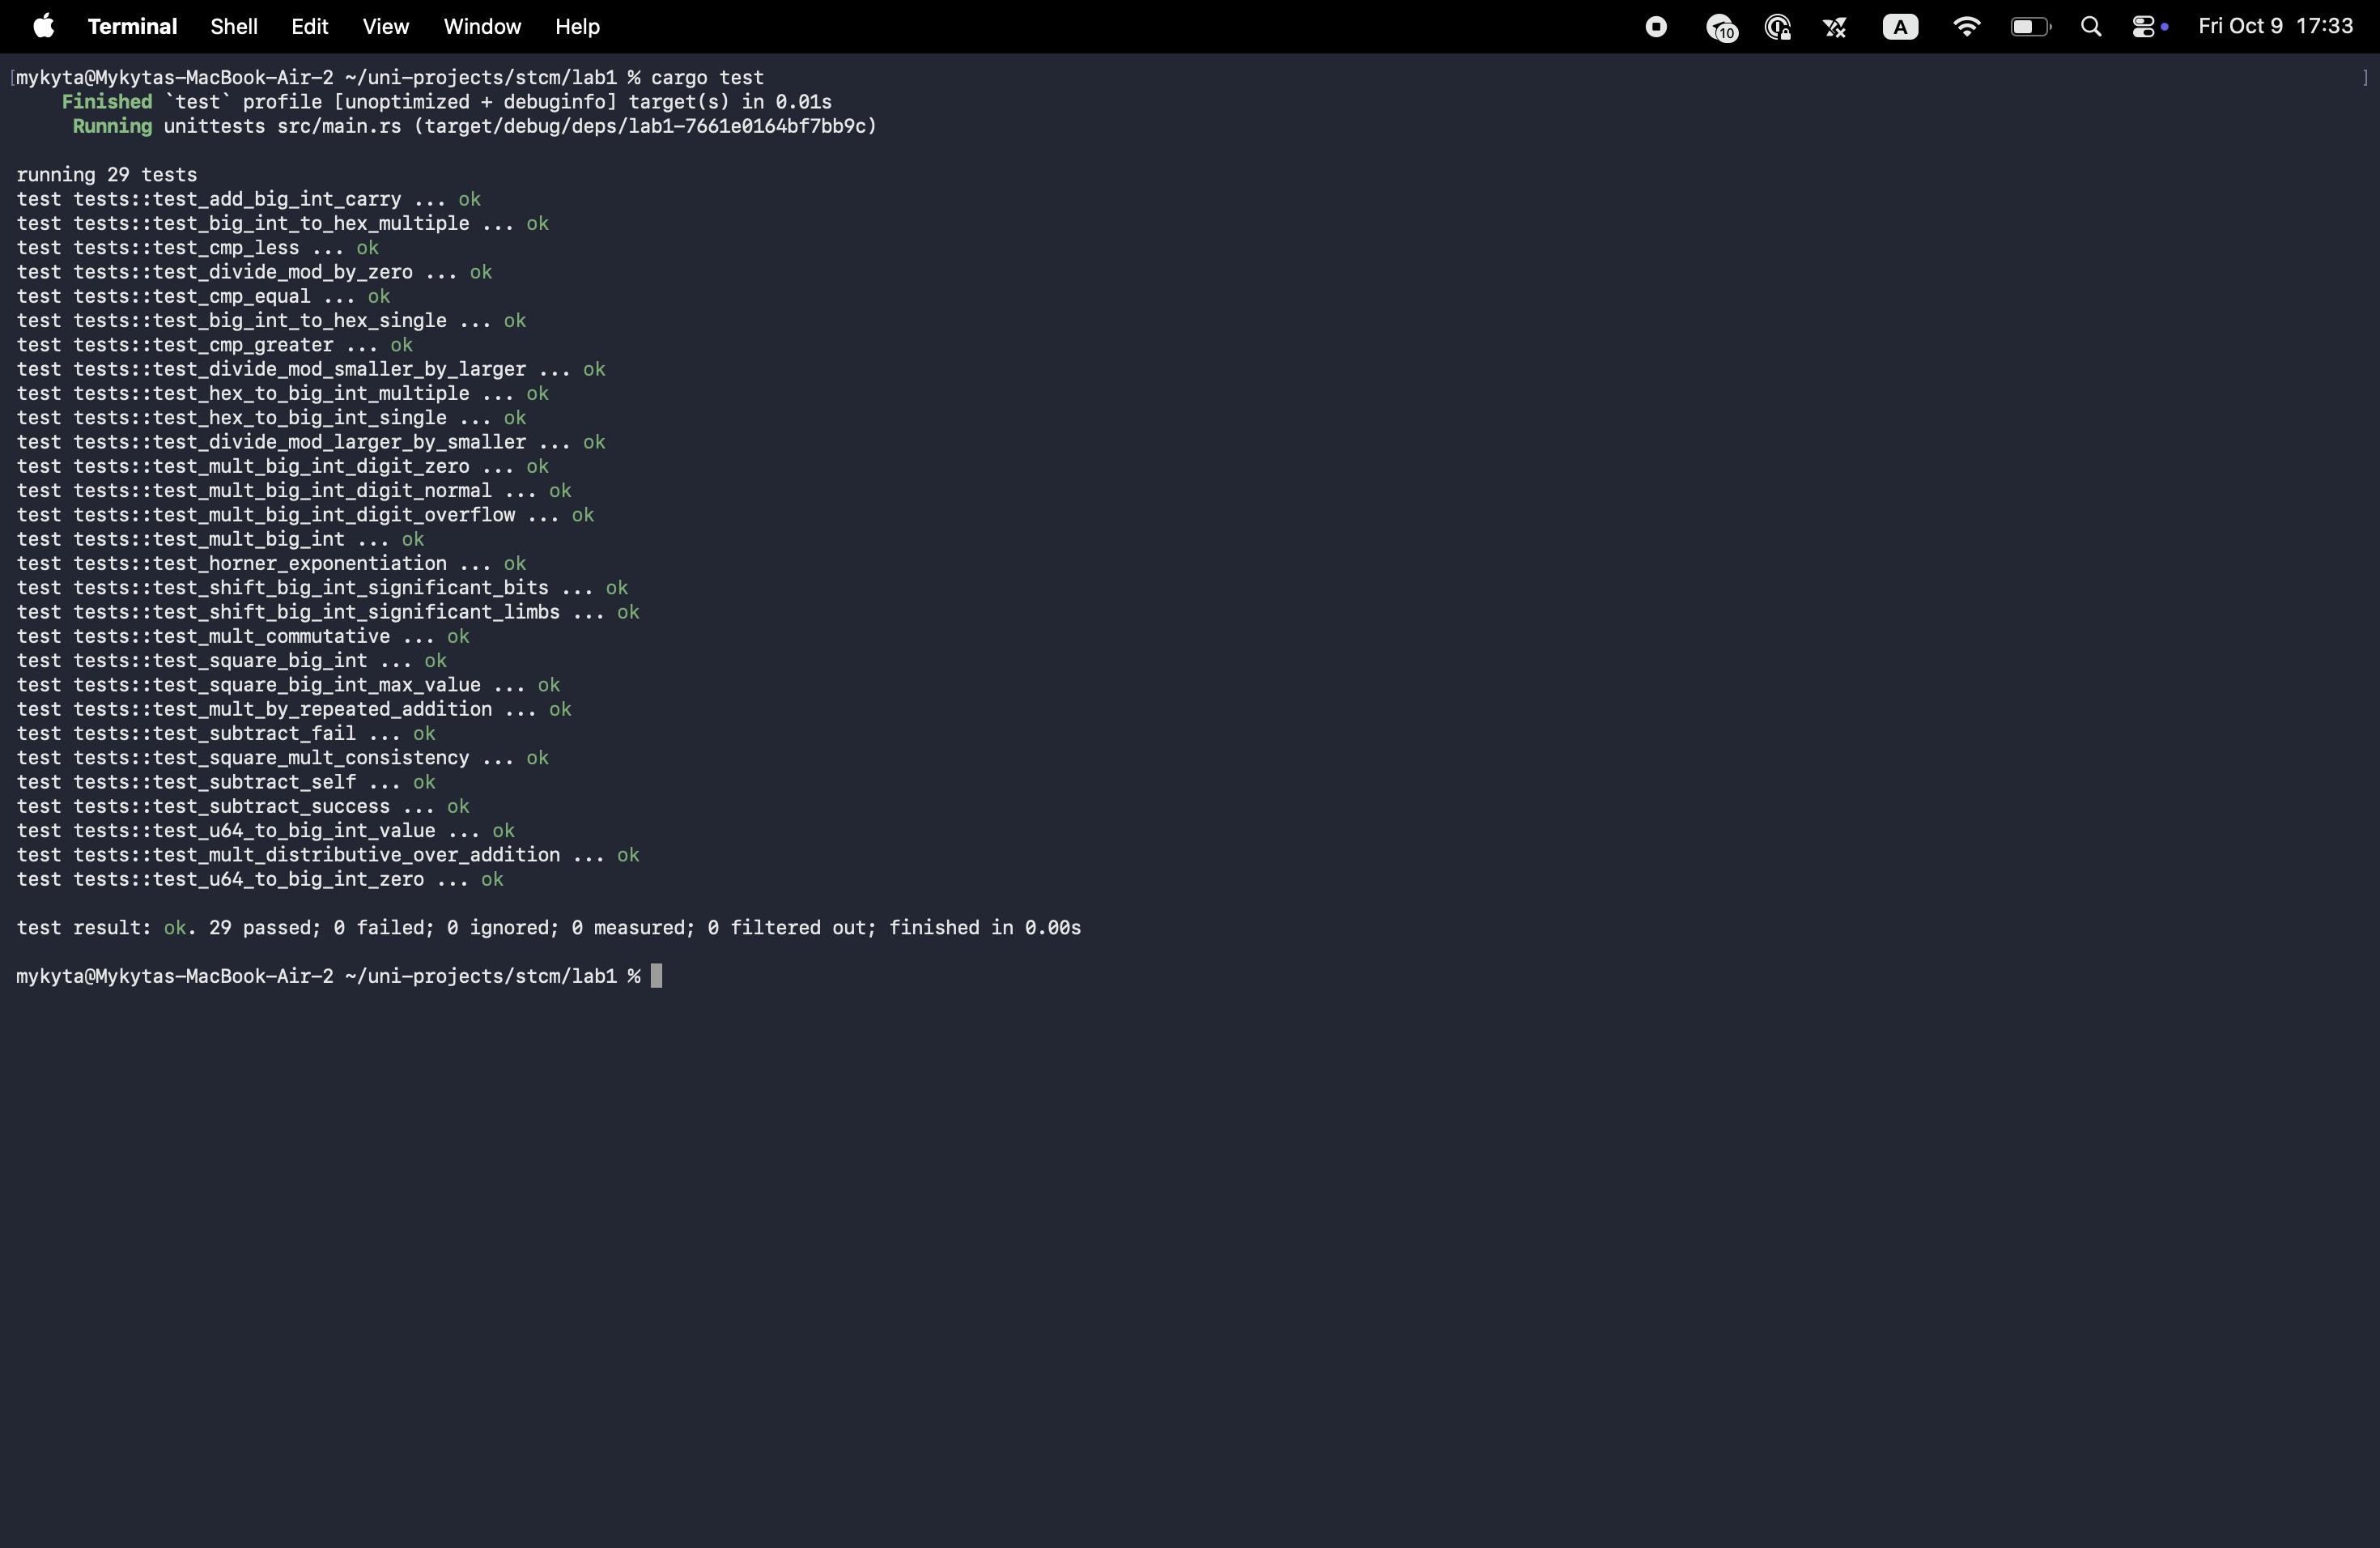
\includegraphics[width=\textwidth]{test-results.png}
    \caption{Успішне виконання тестів}
\end{figure}
\clearpage

\subsection{Результати бенчмарків}

Для кожної операції виконано 1000 прогрівальних запусків, після чого виміряно
середній час для 10000 наборів випадкових вхідних даних. Числа представлені.
Показник часу наведено в наносекундах на одну операцію.
Результати отримано під час запуску оптимізованої release-збірки командою
\code{cargo run --release}.

\noindent\textbf{Додавання}\
78.9 нс/операцію

\medskip
\noindent\textbf{Віднімання}\
52.6 нс/операцію

\medskip
\noindent\textbf{Порівняння}\
4.0 нс/операцію

\medskip
\noindent\textbf{Множення}\
2358.6 нс/операцію

\medskip
\noindent\textbf{Піднесення до квадрата}\
626.3 нс/операцію

\medskip
\noindent\textbf{Ділення та знаходження остачі}\
104.5 нс/операцію

\medskip
\noindent\textbf{Піднесення до степеня методом Горнера}\
10147.0 нс/операцію

\end{document}